% Appendix Template

\chapter{Konfidenzauswertung} % Main appendix title

\label{AppendixF} % Change X to a consecutive letter; for referencing this appendix elsewhere, use \ref{AppendixX}

\begin{figure}[h]
    \centering
    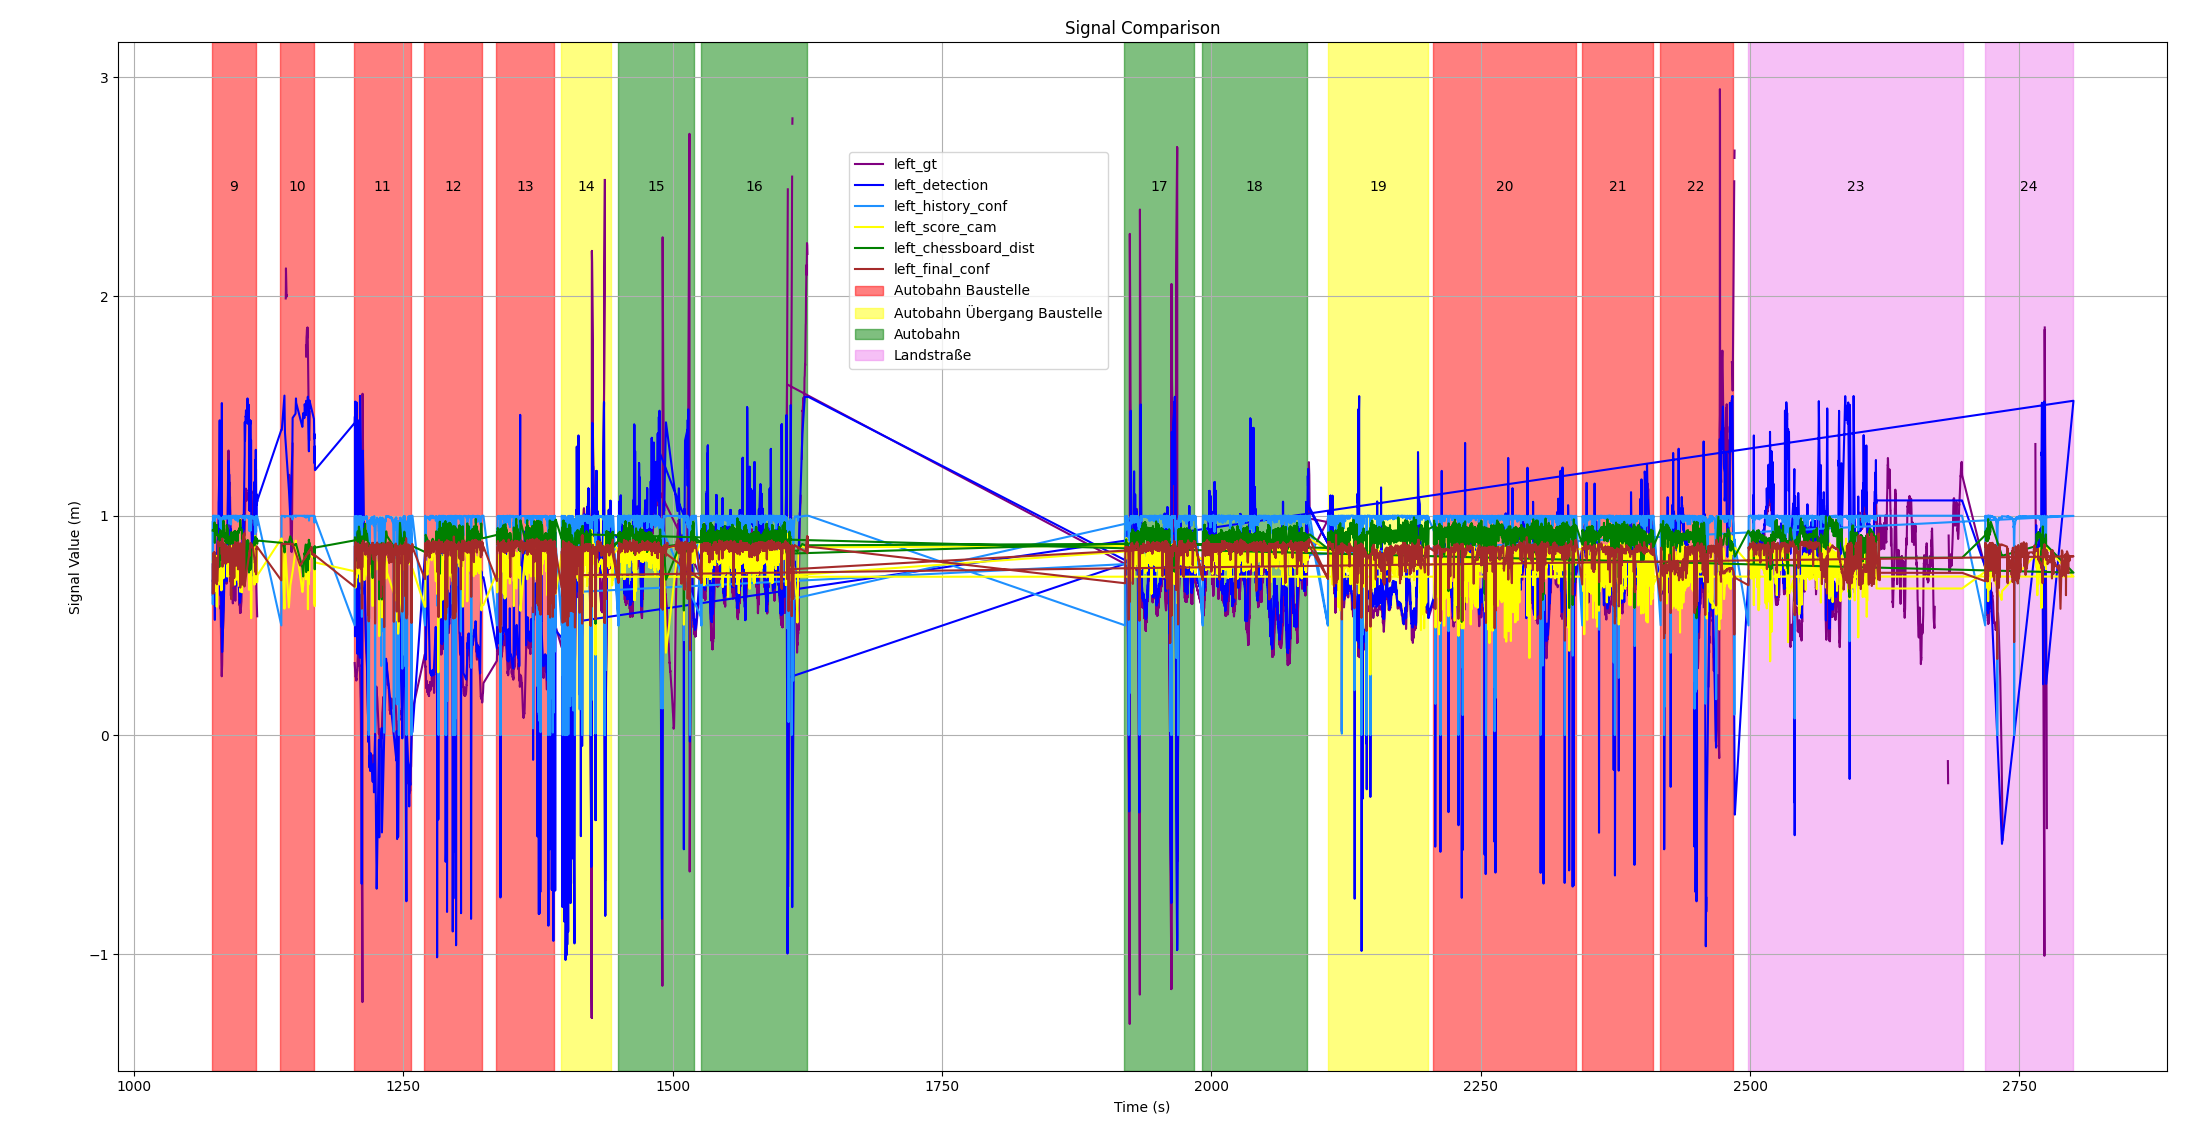
\includegraphics[width=\linewidth]{Figures/M2_left_conf_all.png}
    \caption{Auswertung des Konfidenzwerts Messung 2 links}
    \label{fig:M2_conf_left}
\end{figure}

\begin{figure}[h]
    \centering
    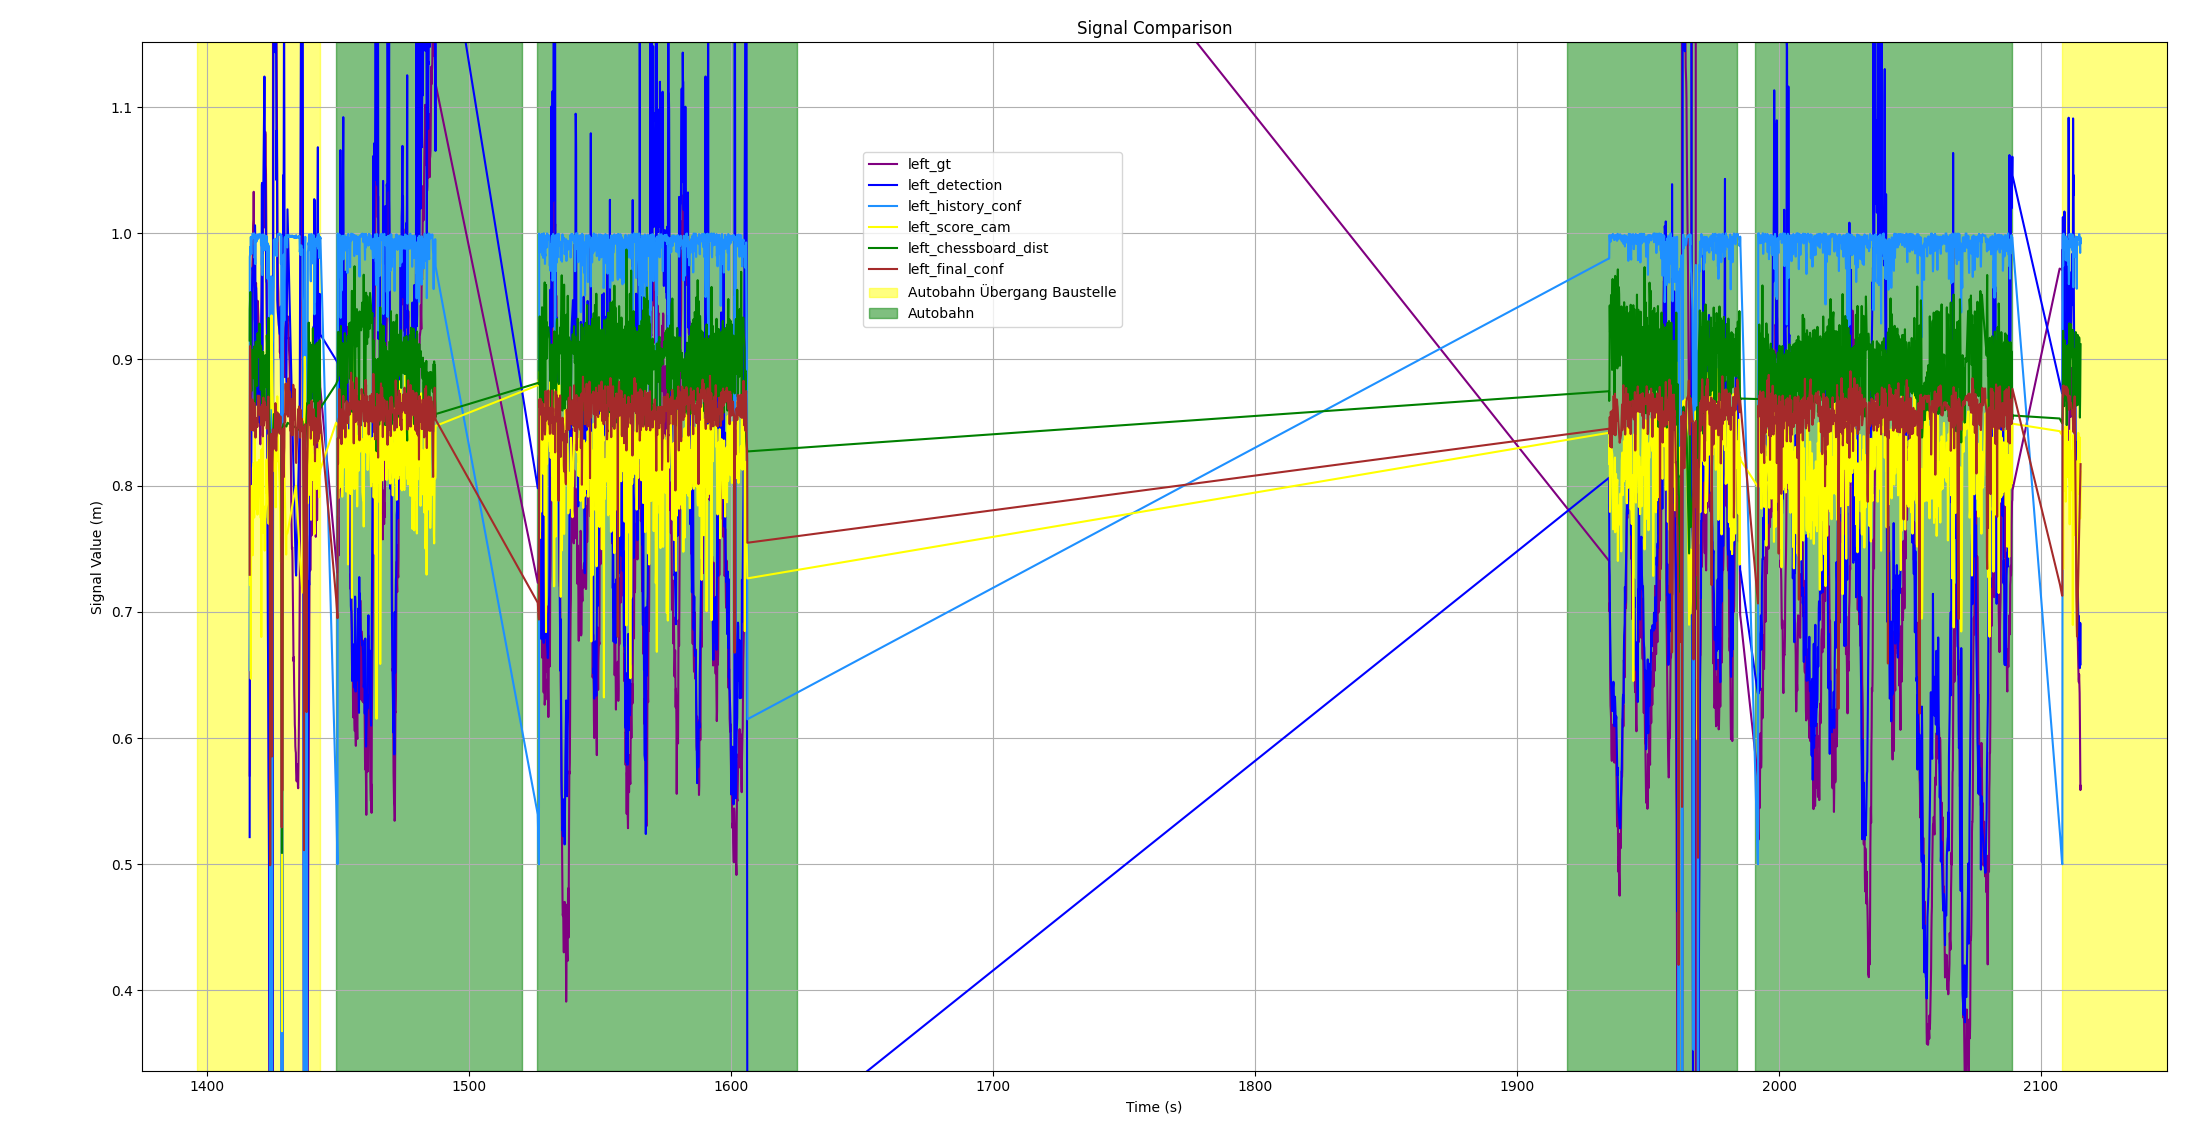
\includegraphics[width=\linewidth]{Figures/M2_left_conf_target_szenario.png}
    \caption{Auswertung des Konfidenzwerts Messung 2 links ohne Sondersituationen}
    \label{fig:M2_conf_left_target}
\end{figure}

\begin{figure}[h]
    \centering
    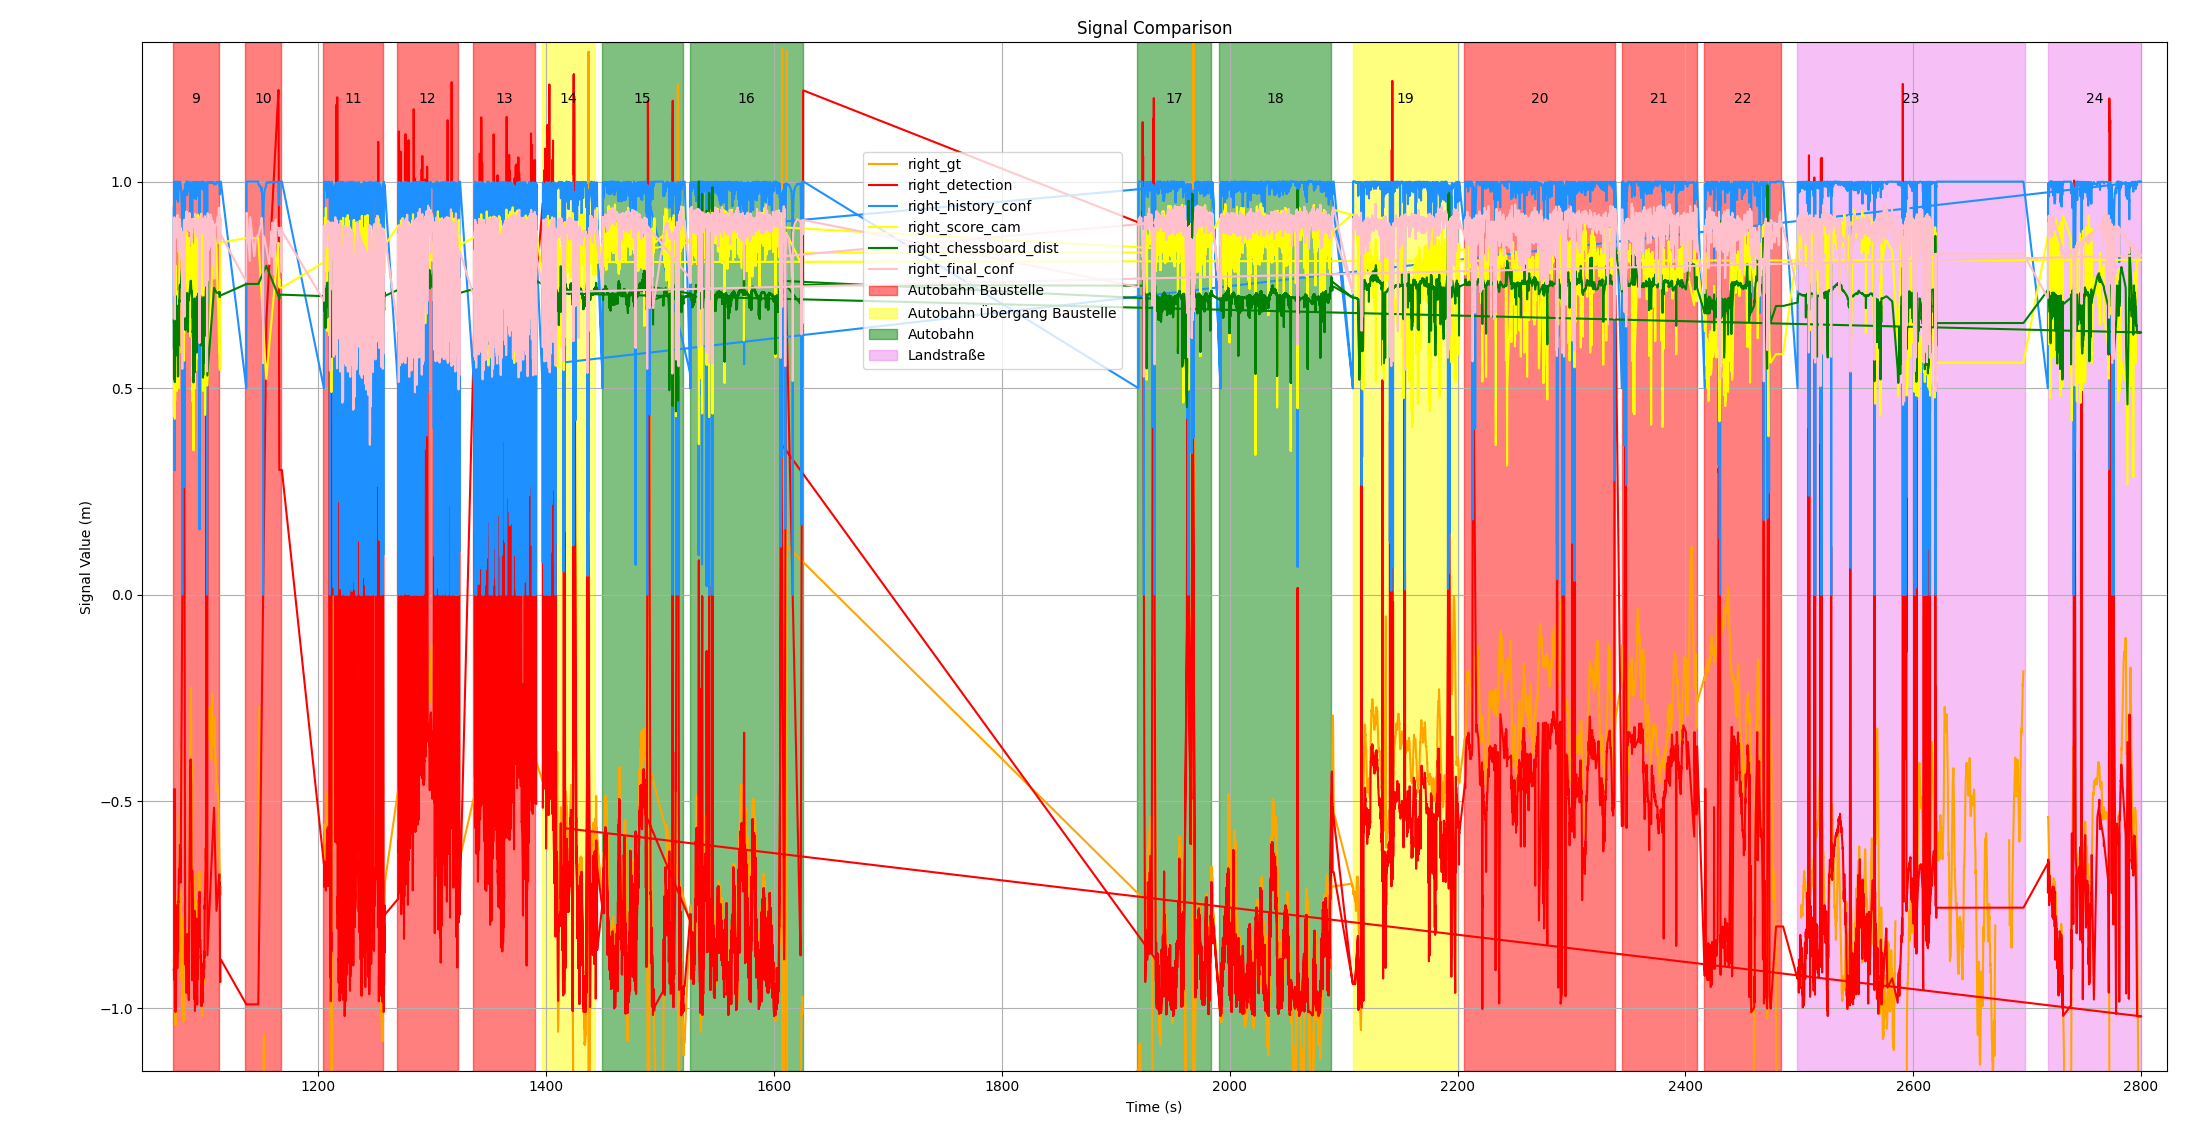
\includegraphics[width=\linewidth]{Figures/M2_right_conf_all.png}
    \caption{Auswertung des Konfidenzwerts Messung 2 rechts}
    \label{fig:M2_conf_right}
\end{figure}

\begin{figure}[h]
    \centering
    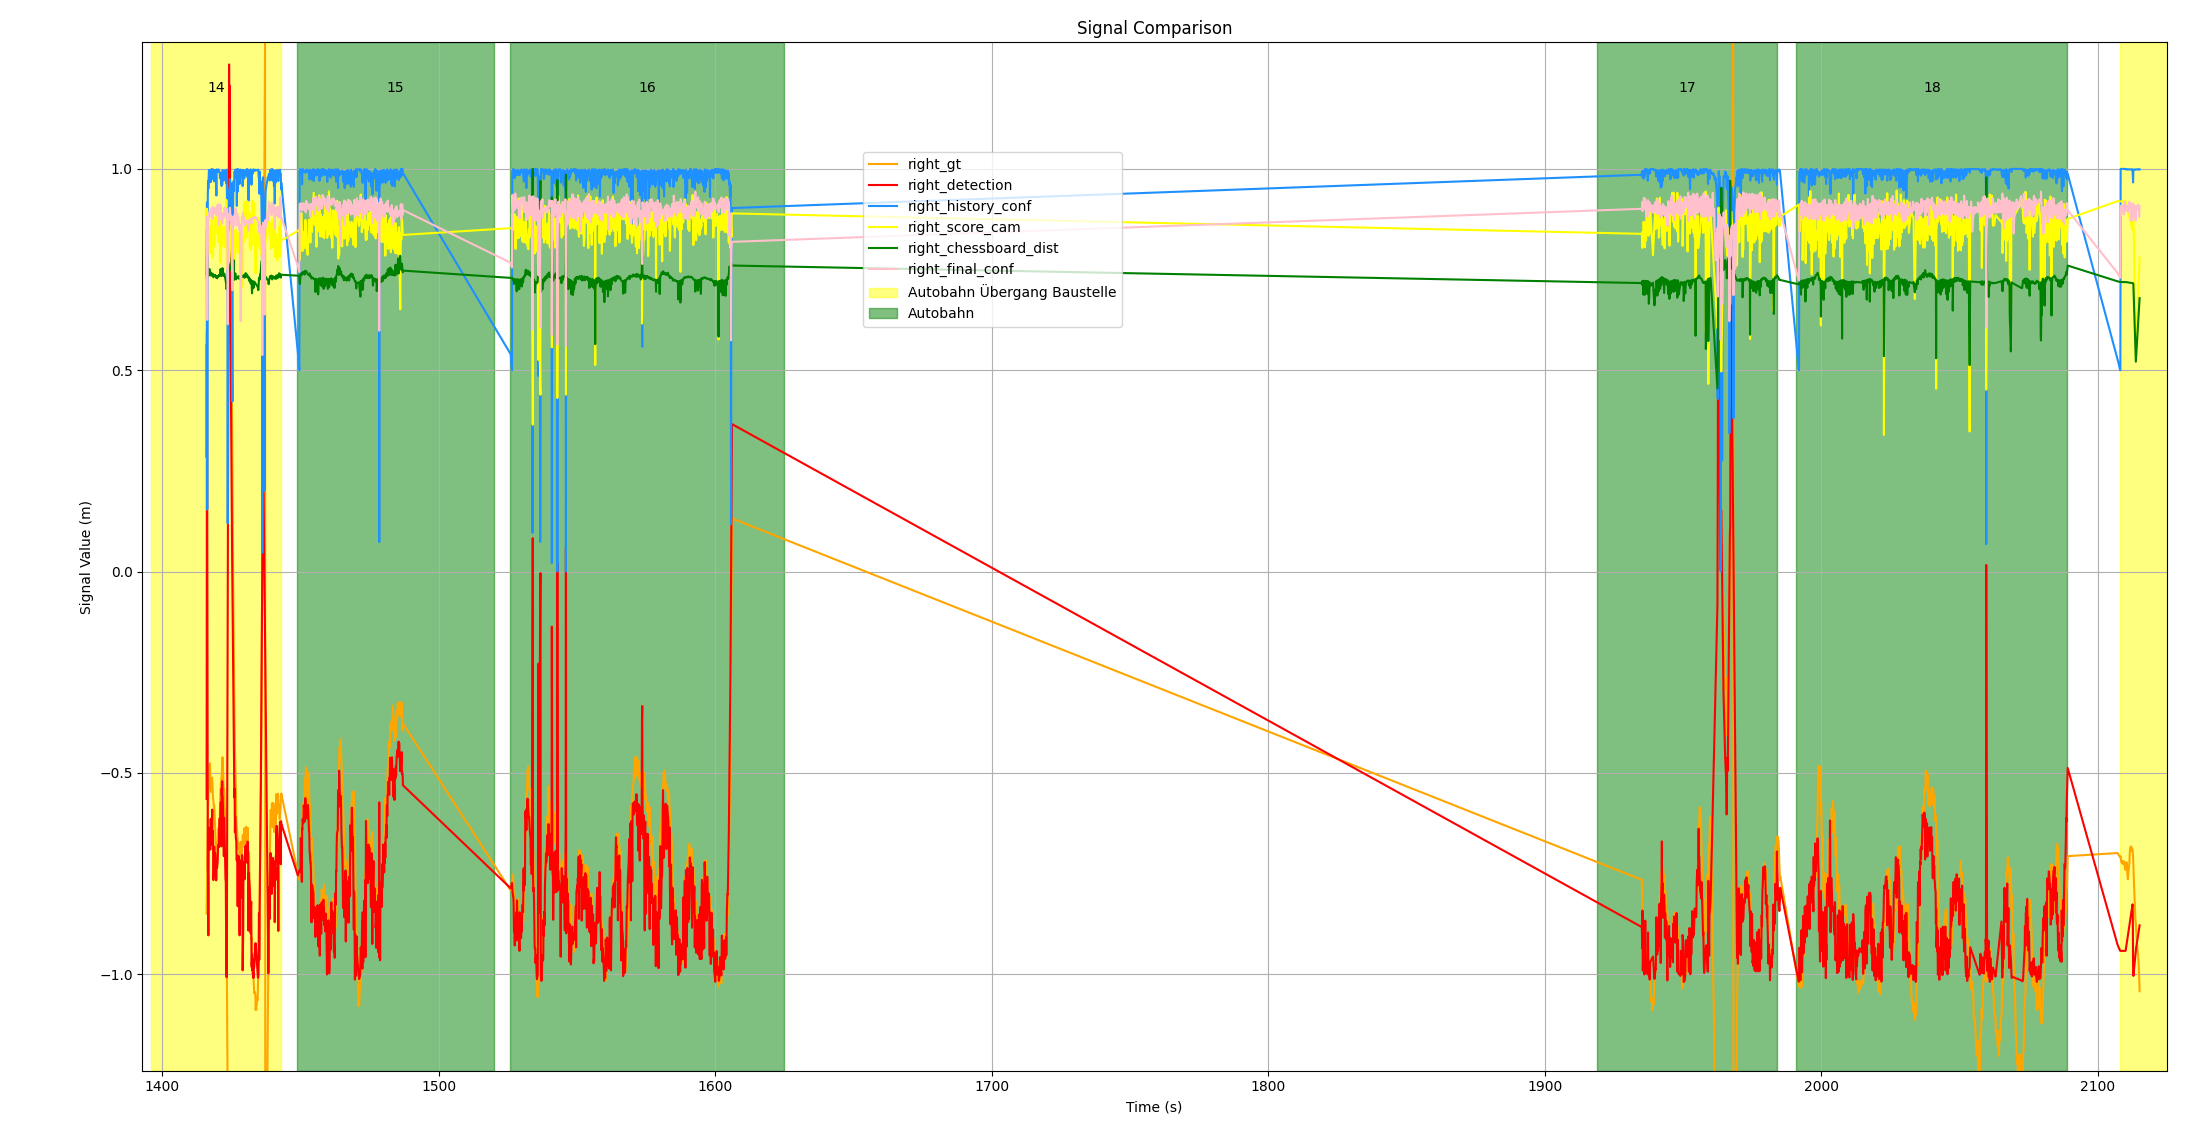
\includegraphics[width=\linewidth]{Figures/M2_right_conf_target_szenario.png}
    \caption{Auswertung des Konfidenzwerts Messung 2 rechts ohne Sondersituationen}
    \label{fig:M2_conf_right_target}
\end{figure}
\clearpage
\begin{figure}[h]
    \centering
    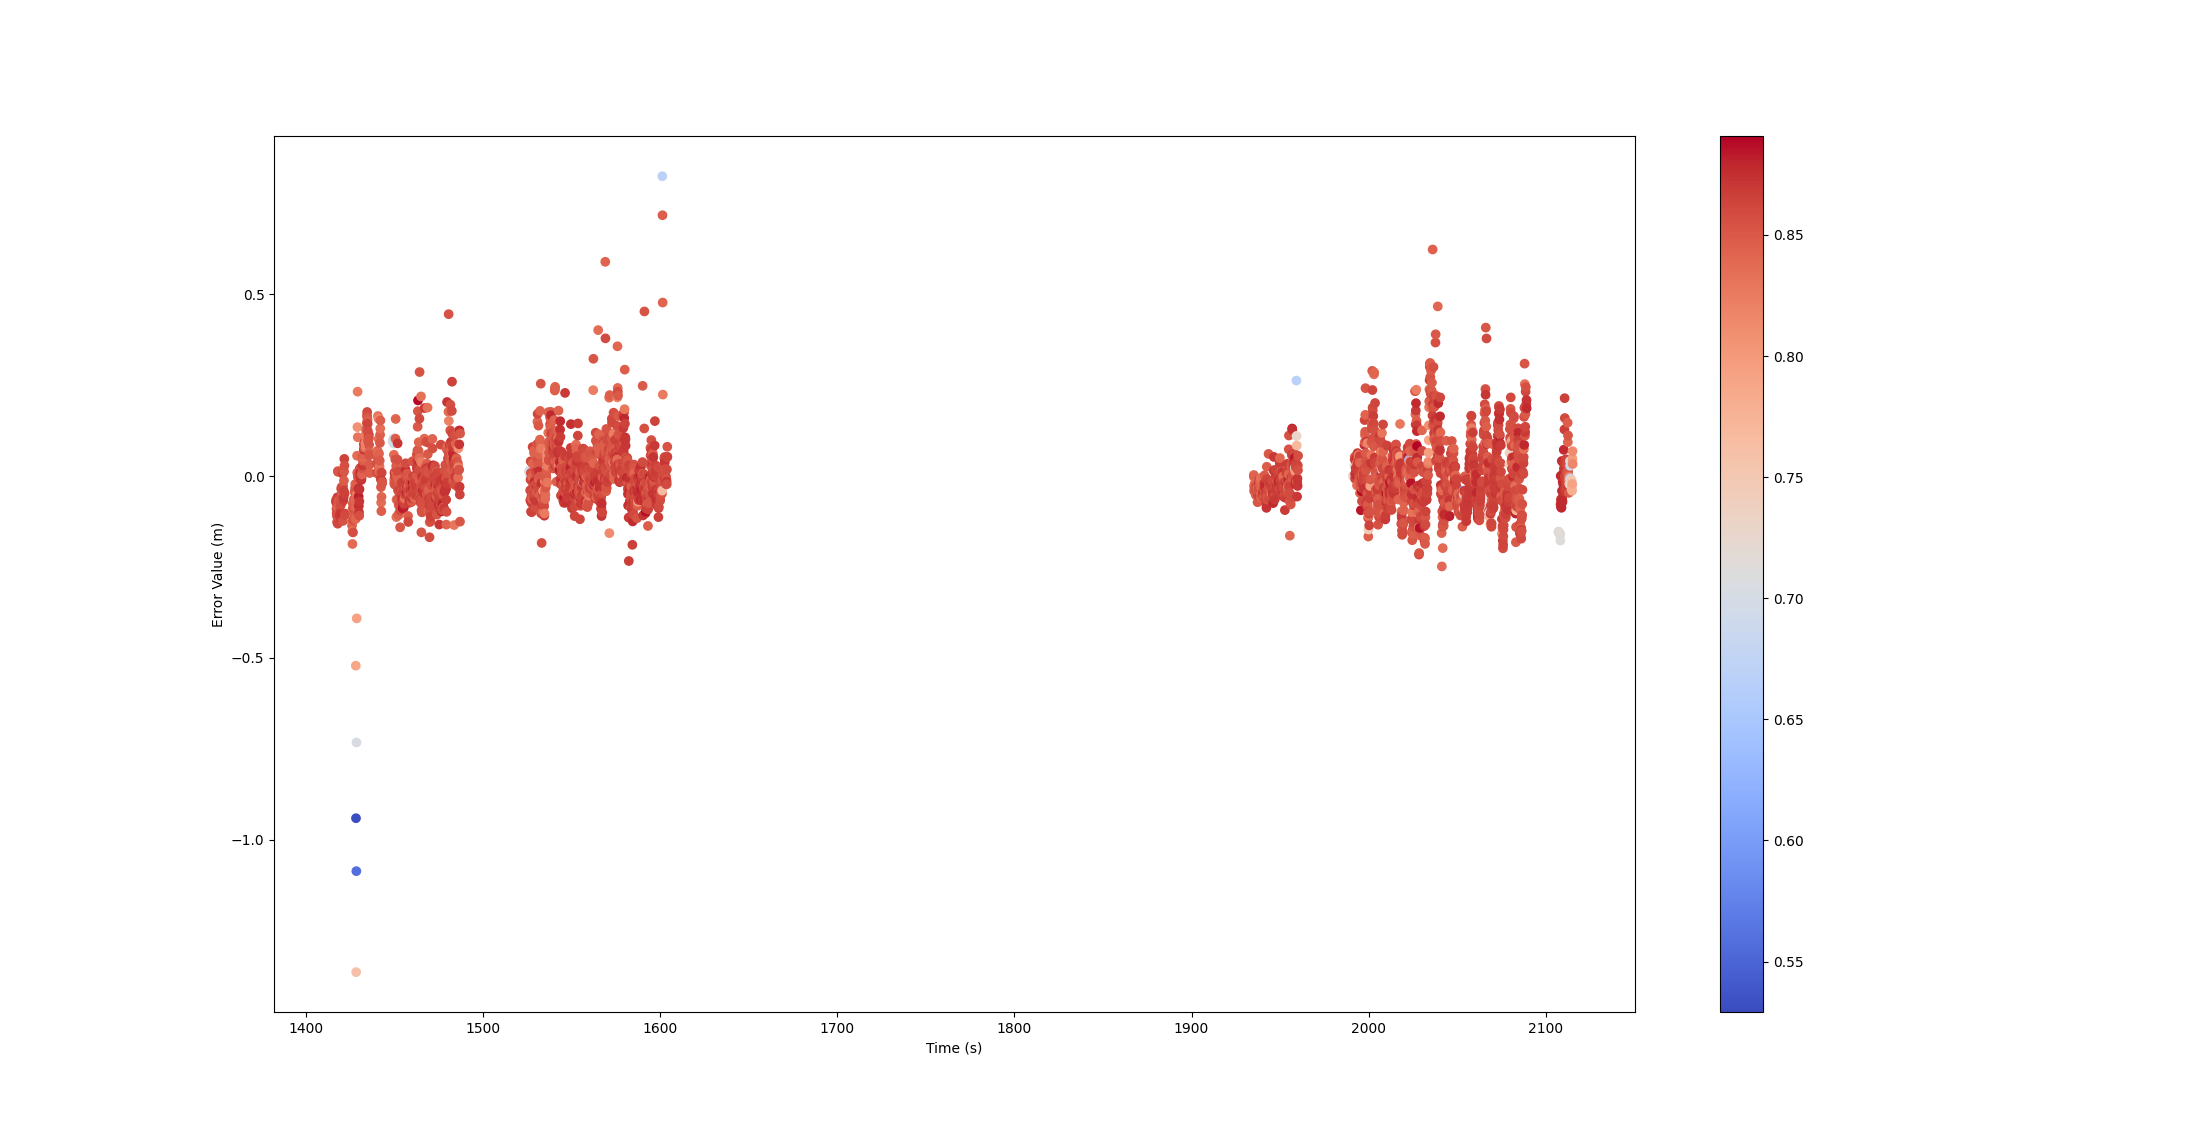
\includegraphics[width=\linewidth]{Figures/M2_left_conf_error_target_szenario.png}
    \caption{Auswertung des Konfidenzwerts Messung 2 links ohne Sondersituationen}
    \label{fig:M2_conf_error_right_target}
\end{figure}

\begin{table}[h]
    \centering
    \begin{tabular}{|c|c|c|c|}
    \hline                      % 68,2%                     % 95,5 %                            % 99,7%
    Konfidenz-Bereich & Fehler in (m) für 1-$\sigma$  & Fehler in (m) für 2-$\sigma$    & Fehler in (m) für 3-$\sigma$    \\
    \hline
    0,9-1,0                 & 0,036                     & 0,11                          & 0,15                         \\
    0,8-0,9                 & 0,051                     & 0,14                          & 0,23                         \\
    0,7-0,8                 & 0,065                     & 0,18                          & 0,28                         \\
    0,6-0,7                 & 0,099                     & 0,26                          & 0,35                         \\
    0,0-0,6                 & 0,625                     & 0,88                          & 1,09                           \\
    
    \hline
    \end{tabular}
    \caption{Verteilung absoluter Fehler in Metern für verschiedene Konfidenz-Bereiche ohne Ausnahmesituationen linke Seite} % 68,3%
    \label{tab:errors_conf_left}
\end{table}

\clearpage

\begin{figure}[h]
    \centering
    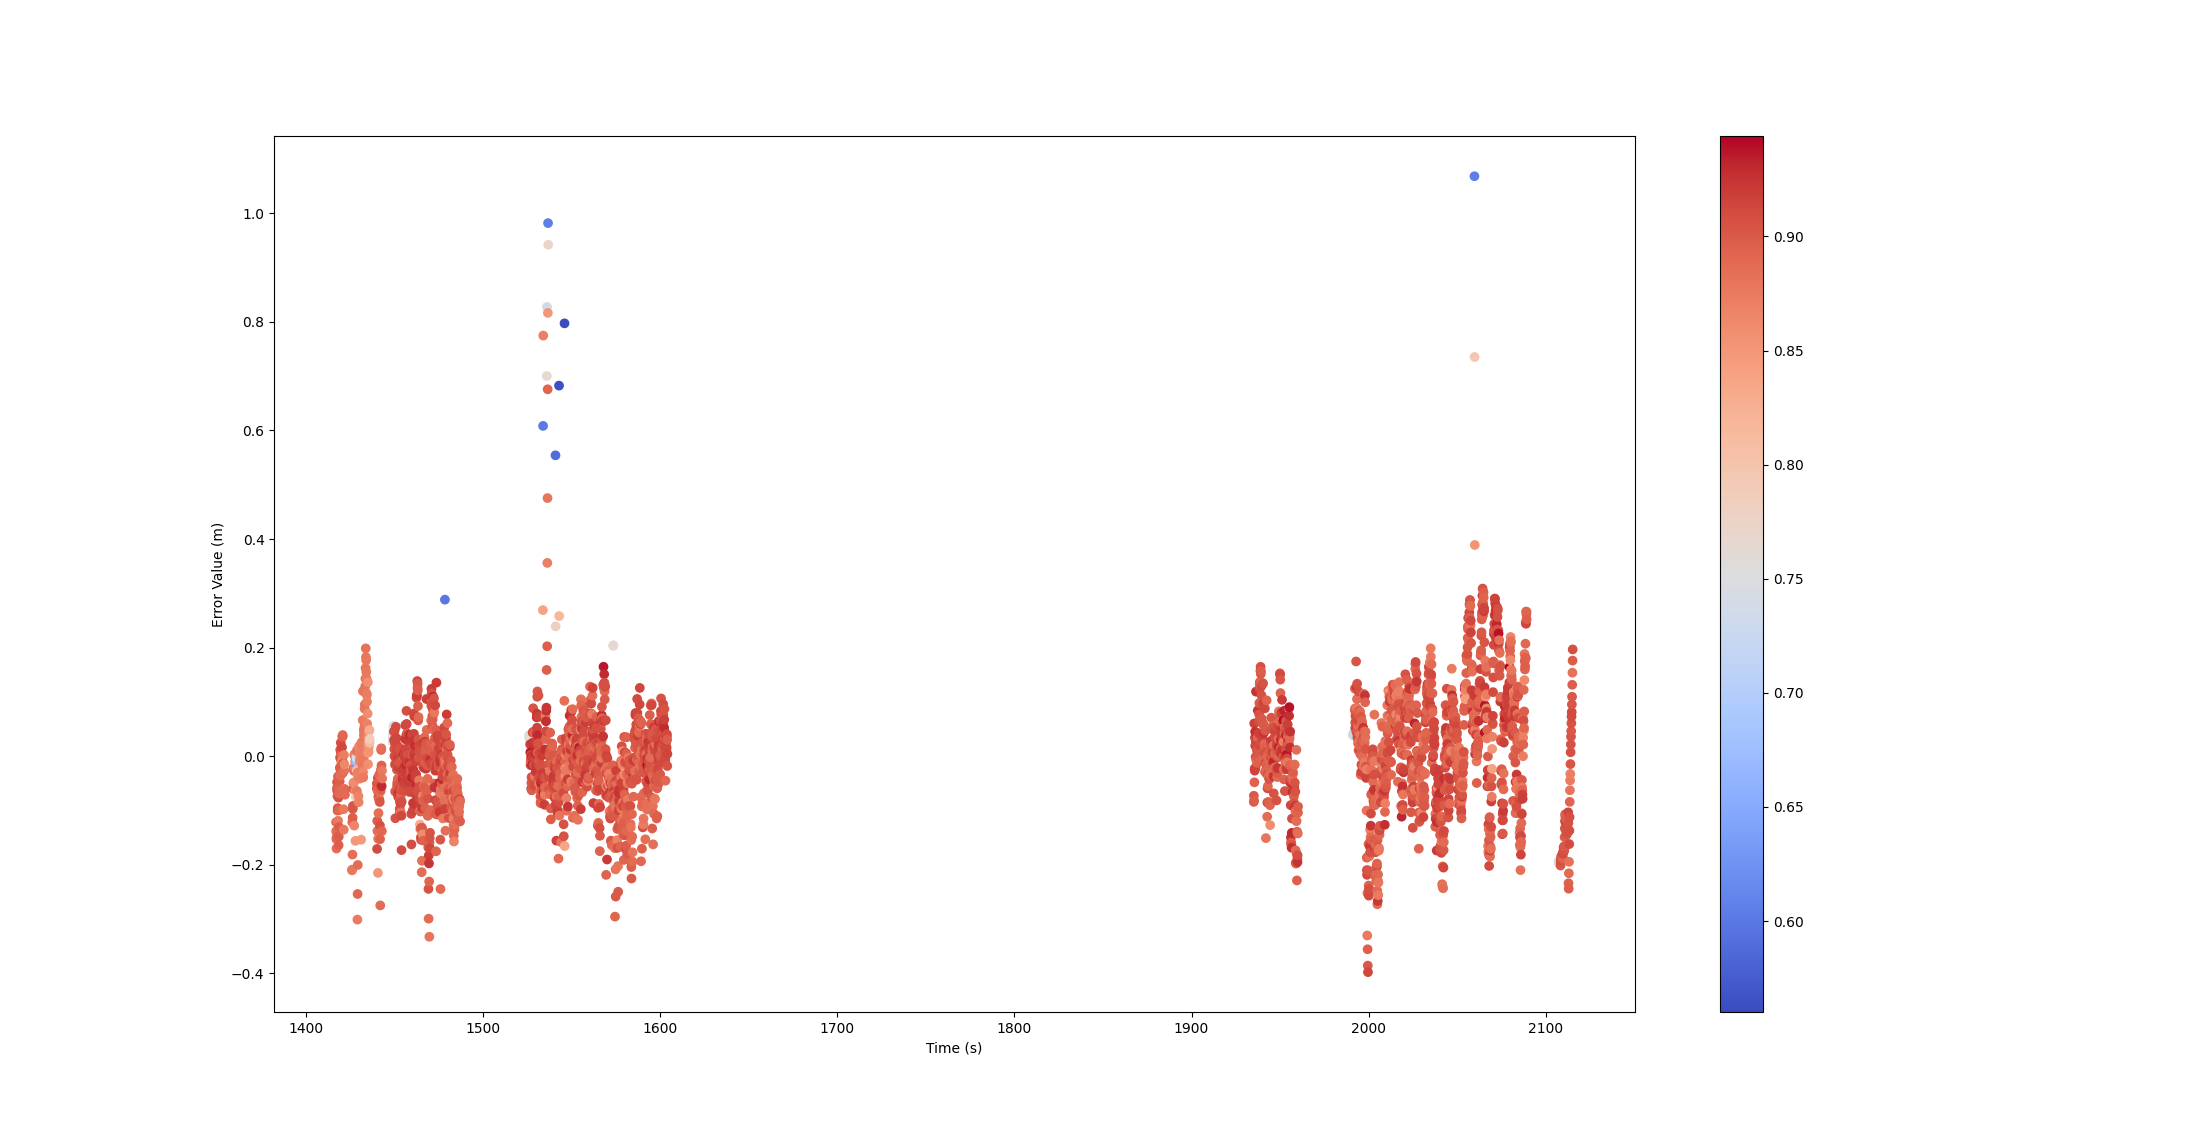
\includegraphics[width=\linewidth]{Figures/M2_right_conf_error_target_szenario.png}
    \caption{Auswertung des Konfidenzwerts Messung 2 rechts ohne Sondersituationen}
    \label{fig:M2_conf_error_left_target}
\end{figure}

\begin{table}[h]
    \centering
    \begin{tabular}{|c|c|c|c|}
    \hline                      % 68,2%                     % 95,5 %                            % 99,7%
    Konfidenz-Bereich & Fehler in (m) für 1-$\sigma$  & Fehler in (m) für 2-$\sigma$    & Fehler in (m) für 3-$\sigma$    \\
    \hline
    0,9-1,0           & 0,062                     & 0,19                          & 0,25                         \\
    0,8-0,9           & 0,087                     & 0,21                          & 0,35                         \\
    0,7-0,8           & 0,108                     & 0,25                          & 0,75                          \\
    0,0-0,7           & 0,742                     & 0,94                          & 1,07                           \\
    
    \hline
    \end{tabular}
    \caption{Verteilung absoluter Fehler in Metern für verschiedene Konfidenz-Bereiche ohne Sondersituationen rechte Seite} % 68,3%
    \label{tab:errors_conf_right}
\end{table}